\section{Leonhard Euler: Mechanics, Rotation, and the Birth of the Moment of Inertia}

\subsection{Evolution of Calculus Notation: From Newton and Leibniz to Euler}

In the decades following the invention of calculus, two competing notational systems vied for prominence.  Leibniz had introduced the symbols
\[
\frac{dy}{dx},\quad \int f(x)\,dx,
\]
treating \(dx\) and \(dy\) as manipulable infinitesimal quantities.  Newton, by contrast, wrote fluxions \( \dot{x} \) and fluents \(x\), anchoring his notation to the notion of absolute time:
\[
\dot{x} = \frac{dx}{dt},\quad x = \int \dot{x}\,dt.
\]
Each system had drawbacks: Leibniz’s differentials offered algebraic flexibility but obscured the underlying function being differentiated, while Newton’s fluxions made the time‐dependence explicit at the cost of generality and ease of composition.

Leonhard Euler bridged these approaches by introducing the explicit function notation and prime‐mark derivatives that underpin modern calculus:
\[
y = f(x),\quad f'(x),\quad f''(x),\quad f^{(n)}(x),
\]
while retaining Leibniz’s \(d\) notation for differentials and integrals.  Euler’s innovation clarified which variable was changing, permitted concise expression of higher‐order derivatives, and allowed power‐series and transcendental functions to be treated uniformly.

With this unified notation in hand—combining the algebraic strength of Leibniz’s \(d\) and \(\int\) with Euler’s function‐and‐prime conventions—we are prepared to explore how Euler extended calculus beyond straight‐line motion into the mechanics of rotation.  


\begin{figure}[H]
    \centering
    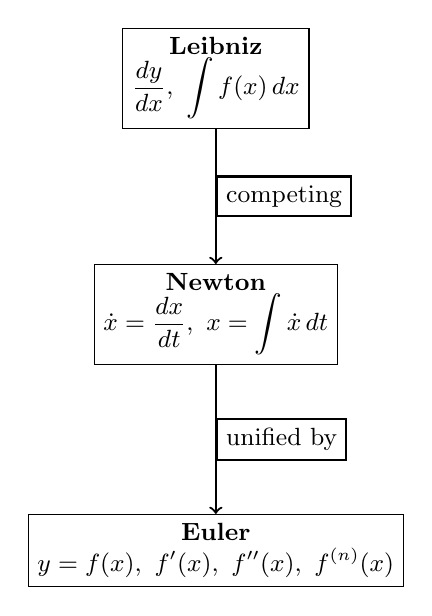
\begin{tikzpicture}[
        every node/.style={draw, rectangle, align=center, font=\small},
        node distance=3cm
      ]
      % Nodes for each notation system, stacked vertically
      \node (Leibniz) {%
        \textbf{Leibniz}\\
        $\displaystyle \frac{dy}{dx},\ \int f(x)\,dx$%
      };
      \node (Newton) [below of=Leibniz] {%
        \textbf{Newton}\\
        $\displaystyle \dot{x} = \frac{dx}{dt},\ x = \int \dot{x}\,dt$%
      };
      \node (Euler) [below of=Newton] {%
        \textbf{Euler}\\
        $y = f(x),\ f'(x),\ f''(x),\ f^{(n)}(x)$%
      };
  
      % Arrows indicating the evolution
      \draw[->, thick] (Leibniz) -- node[right]{competing} (Newton);
      \draw[->, thick] (Newton) -- node[right]{unified by} (Euler);
    \end{tikzpicture}
    \caption{Evolution of calculus notation: from Leibniz’s infinitesimals and integrals, through Newton’s fluxions and fluents, to Euler’s function‐and‐prime conventions.}
    \label{fig:calculus-notation-evolution}
\end{figure}
  


\subsection{Euler’s Notational Reform and the Algebra of Optimization}


If Newton gave us the calculus of straight‐line motion, and Leibniz gave us the calculus of relations, then \textbf{Leonhard Euler} extended both the notation and the scope of calculus.

Euler not only carried calculus into rotation, he also reframed how we approach optimization.  Whereas Leibniz located extrema by manipulating infinitesimal differentials—
\[
df = 0\quad\bigl(\tfrac{dy}{dx}=0\bigr),
\]
Euler introduced explicit function notation and the prime‐mark derivative:
\[
y = f(x),\qquad f'(x) = 0.
\]
Optimization thus became the algebraic task of solving the equation \(f'(x)=0\), with the infinitesimals \(dx, dy\) safely hidden behind a cleaner \(f'\) notation.  This shift didn’t abandon Leibniz’s infinitesimals so much as streamline them into the background, turning “optimize the infinitesimal threads” into “optimize the function” in a single symbolic step.

For Euler, motion wasn’t limited to points sliding along curves—it also involved bodies spinning, tumbling, and twisting through space.  Where Newton’s laws explained how objects move in straight paths under forces, Euler asked:

\begin{quote}
\textit{How do extended bodies rotate? How do we measure their resistance to being spun?}
\end{quote}

This question led him to one of his most enduring contributions: the concept of the \textbf{moment of inertia}.  


\begin{figure}[H]
    \centering
    \begin{tikzpicture}[
        node distance=4cm,
        box/.style={
          draw, rectangle, rounded corners,
          align=center, font=\small,
          minimum width=4cm, minimum height=2cm
        },
        >=stealth
      ]
      % Nodes stacked vertically
      \node[box] (Leibniz) {
        \textbf{Leibniz’s View}\\
        Infinitesimal threads\\
        \(\displaystyle df = 0\)\\
        \(\displaystyle \tfrac{dy}{dx} = 0\)
      };
      \node[box] (Euler) [below of=Leibniz] {
        \textbf{Euler’s Reform}\\
        Function‐and‐prime notation\\
        \(\displaystyle y = f(x)\)\\
        \(\displaystyle f'(x) = 0\)
      };
  
      % Arrow pointing downward
      \draw[->, thick] (Leibniz.south) -- node[midway,right]{Reframed by Euler} (Euler.north);
    \end{tikzpicture}
    \caption{Optimization in Leibniz’s infinitesimal calculus (\(df=0\)) versus Euler’s algebraic calculus (\(f'(x)=0\)).}
    \label{fig:leibniz-euler-optimization-vertical}
\end{figure}
  



\subsection{A New Quantity for Rotating Bodies}

Imagine trying to spin a wheel. Intuitively, you know it’s harder to spin a heavy wheel than a light one. But 
it’s also harder to spin a wheel if more of its mass is far from the center. A solid disc and a bicycle rim 
might weigh the same, but the rim resists spinning more.

Euler formalized this intuition with a mathematical expression that measured how mass is distributed relative 
to an axis of rotation. He defined the moment of inertia \( I \) as:

\[
I = \sum m_i r_i^2
\]

where:

\begin{itemize}
    \item \( m_i \) is the mass of each particle in the body,
    \item \( r_i \) is the distance of that particle from the axis of rotation.
\end{itemize}

This formula told physicists and engineers something profound:  
\textbf{Not all mass contributes equally to rotational inertia; distance matters quadratically.}

\begin{figure}[H]
    \centering
    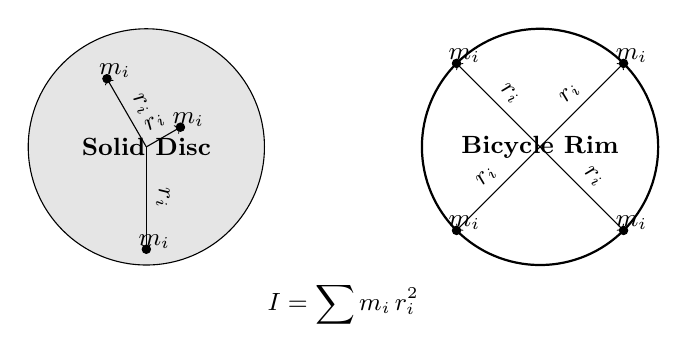
\begin{tikzpicture}[scale=1, every node/.style={font=\small}]
      % Solid disc
      \begin{scope}
        \filldraw[fill=gray!20, draw=black] (0,0) circle (1.5cm);
        \node at (0,0) [font=\small\bfseries] {Solid Disc};
        % Sample mass points at various radii
        \foreach \angle/\rad in {30/0.5, 120/1.0, 270/1.3} {
          \filldraw[black] (\angle:\rad) circle (1.5pt) node[shift={(0.1,0.1)}] {$m_i$};
          \draw[->] (0,0) -- (\angle:\rad) node[midway, sloped, above] {$r_i$};
        }
      \end{scope}
  
      % Bicycle rim
      \begin{scope}[xshift=5cm]
        \draw[thick] (0,0) circle (1.5cm);
        \node at (0,0) [font=\small\bfseries] {Bicycle Rim};
        % Sample mass points all at outer radius
        \foreach \angle in {45, 135, 225, 315} {
          \filldraw[black] (\angle:1.5) circle (1.5pt) node[shift={(0.1,0.1)}] {$m_i$};
          \draw[->] (0,0) -- (\angle:1.5) node[midway, sloped, above] {$r_i$};
        }
      \end{scope}
  
      % Formula annotation
      \node at (2.5,-2) {\(\displaystyle I = \sum m_i\,r_i^2\)};
    \end{tikzpicture}
    \caption{Comparison of mass distributions: a uniformly filled disc versus a rim with all mass at the edge.  The moment of inertia \(I=\sum m_ir_i^2\) is larger for the rim, since its mass elements sit at greater \(r_i\).}
    \label{fig:moment-of-inertia-distribution}
\end{figure}


In continuous terms, for a solid body:

\[
I = \int r^2 \, dm
\]

Here, \( r \) measures the perpendicular distance from each infinitesimal mass element \( dm \) to the axis.

\begin{figure}[H]
    \centering
    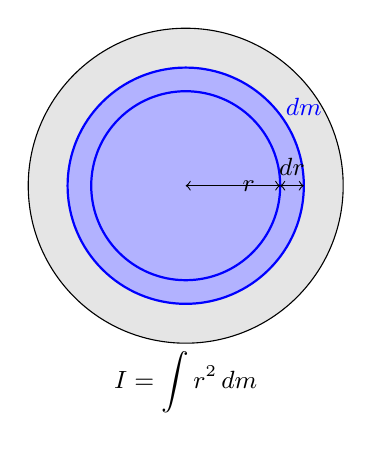
\begin{tikzpicture}[scale=1, every node/.style={font=\small}]
      % Parameters
      \def\R{2}     % outer radius of the body
      \def\r{1.2}   % radius of the infinitesimal ring
      \def\dr{0.3}  % thickness of the ring
  
      % Draw full body (cross‐section)
      \filldraw[fill=gray!20, draw=black] (0,0) circle (\R);
  
      % Highlight infinitesimal ring dm
      \fill[blue!30]
        (0,0) circle (\r + \dr)
        (0,0) circle (\r)
        rectangle ++(0,0); % even‐odd rule
  
      % Draw ring boundary
      \draw[blue, thick] (0:\r) arc (0:360:\r);
      \draw[blue, thick] (0:{\r+\dr}) arc (0:360:{\r+\dr});
  
      % Arrows and labels for r and dr
      \draw[<->] (0,0) -- node[midway, right] {$r$} (\r,0);
      \draw[<->] ({\r},0) -- node[midway, above] {$dr$} ({\r+\dr},0);
  
      % Label for dm
      \node[blue] at (1.5,1.0) {$dm$};
  
      % Integral formula annotation
      \node at (0,-2.5) {\(\displaystyle I = \int r^2\,dm\)};
    \end{tikzpicture}
    \caption{Infinitesimal ring element at radius \(r\) with thickness \(dr\) and mass \(dm\), illustrating the continuous definition \(I = \int r^2\,dm\) of the moment of inertia.}
    \label{fig:moment-of-inertia-continuous}
\end{figure}


\begin{HistoricalSidebar}{Why “Inertia”?}

The term “moment of inertia” reflects a conceptual bridge: it extends Newton’s linear inertia 
(resistance to acceleration) into the rotational domain.

Just as force produces linear acceleration in proportion to mass, a torque (rotational force) 
produces angular acceleration in proportion to moment of inertia:

\[
\tau = I \alpha
\]

Euler’s insight was to see inertia not as a single number, but as a geometric property: how mass is 
distributed around an axis shapes a body’s resistance to rotational change.

\end{HistoricalSidebar}

\subsection{Euler’s Equations of Rigid Body Rotation}

Euler formulated the motion of a rigid body by resolving it about its principal axes, with principal moments of inertia \(A\), \(B\), \(C\) and angular velocity components \(\omega_{1}\), \(\omega_{2}\), \(\omega_{3}\).  Denoting the external torques about these axes by \(M_{1}\), \(M_{2}\), \(M_{3}\), he showed that

\[
\begin{aligned}
A\,\frac{d\omega_{1}}{dt} + (C - B)\,\omega_{2}\,\omega_{3} &= M_{1},\\
B\,\frac{d\omega_{2}}{dt} + (A - C)\,\omega_{3}\,\omega_{1} &= M_{2},\\
C\,\frac{d\omega_{3}}{dt} + (B - A)\,\omega_{1}\,\omega_{2} &= M_{3}.
\end{aligned}
\]

These are \emph{Euler’s equations of motion} for a spinning rigid body.  He derived them by equating the time‐rate‐of‐change of each component of angular momentum \(A\omega_{1}\), \(B\omega_{2}\), \(C\omega_{3}\) to the corresponding applied torque, entirely in terms of the principal moments and angular velocity components—long before any modern tensor language existed.  

\begin{figure}[H]
    \centering
    \begin{tikzpicture}[scale=1, every node/.style={font=\small}, >=stealth]
      % Define origin and axes endpoints
      \coordinate (O) at (0,0);
      \coordinate (X) at (3,0);
      \coordinate (Y) at (0,3);
      \coordinate (Z) at (-1.5,1.5);
  
      % Draw principal axes
      \draw[->] (O) -- (X) node[right] {$x$};
      \draw[->] (O) -- (Y) node[above] {$y$};
      \draw[->] (O) -- (Z) node[above left] {$z$};
  
      % Angular velocity components ω_i
      \draw[->, thick, blue] (O) -- ($(O)!0.7!(X)$) node[midway,below] {$\omega_{1}$};
      \draw[->, thick, blue] (O) -- ($(O)!0.7!(Y)$) node[midway,left]  {$\omega_{2}$};
      \draw[->, thick, blue] (O) -- ($(O)!0.7!(Z)$) node[midway,above left] {$\omega_{3}$};
  
      % Applied torques M_i (dashed red)
      \draw[->, thick, red, dashed] (O) -- ($(O)!0.5!(X)$) node[midway,above] {$M_{1}$};
      \draw[->, thick, red, dashed] (O) -- ($(O)!0.5!(Y)$) node[midway,right] {$M_{2}$};
      \draw[->, thick, red, dashed] (O) -- ($(O)!0.5!(Z)$) node[midway,below left] {$M_{3}$};
  
      % Principal moments labels
      \node at ($(O)!0.9!(X)$)[above right] {$A$};
      \node at ($(O)!0.9!(Y)$)[above left]  {$B$};
      \node at ($(O)!0.9!(Z)$)[below left]  {$C$};
    \end{tikzpicture}
    \caption{Principal axes of a rigid body with angular velocity components $\omega_i$, applied torques $M_i$, and principal moments of inertia $A,B,C$.}
    \label{fig:euler-rigid-body-axes}
\end{figure}



\subsection{A World Beyond Points}

Euler’s contributions shifted mechanics from the study of point masses to the study of extended bodies. His 
moment of inertia allowed physicists to calculate how real objects spin, from gears to planets.

Where Newton gave us forces and fluxions, and Leibniz gave us differentials and optimization, Euler connected 
their ideas to the practical mechanics of the physical world:

\begin{center}
\begin{tabular}{c|c|c}
\textbf{Newton} & \textbf{Leibniz} & \textbf{Euler} \\
\hline
Force & Relation & Rotation \\
Fluxion & Differential & Moment of Inertia \\
Absolute Time & Algebraic Structure & Geometric Distribution \\
\end{tabular}
\end{center}

Euler turned motion from an abstract flow or a symbolic ratio into an engineering toolkit.

\begin{HistoricalSidebar}{Euler and the Calculus of Rotating Worlds}
  
Leonhard Euler wasn’t simply expanding calculus—he was expanding its domain. With his moment of inertia 
and rotational dynamics, he allowed calculus to describe not just paths, but \textbf{bodies spinning around axes}, 
tumbling in space, balancing forces.

\medskip

Euler’s work laid the foundation for structural engineering, celestial mechanics, and modern physics. His 
equations are still taught to every engineer and physicist who studies rotation.

\medskip

In a universe of spinning planets, rolling wheels, and orbiting moons, Euler gave calculus a new playground: 
the rotating world.

\end{HistoricalSidebar}

\subsection{The Legacy of Inertia}

Today, the moment of inertia appears in everything from gymnasts adjusting their spin mid-air to 
satellites controlling their orientation in space.

Whenever we write:

\[
\tau = I \alpha
\]

—or calculate how a shape’s geometry affects its spin—we invoke Euler’s insight.

Euler’s mechanics didn’t replace Newton’s. It extended it into dimensions Newton never charted: the rotational, 
the distributed, the tensorial.

Where Newton saw the flow of time, and Leibniz saw the grammar of infinitesimals, Euler saw the shape of 
things that spin—and gave us the mathematics to set them in motion.

\subsection{Kepler’s Second Law Reimagined: Moment of Inertia and Angular Momentum}

Newton had shown that Kepler’s Second Law—the law of equal areas swept in equal times—was a consequence 
of a central force. But with Euler’s insight into rotational dynamics, we can reinterpret this geometric 
law in a new light: as the conservation of \textbf{angular momentum}.

Consider a planet orbiting the Sun. At each moment:

\[
L = I \omega
\]

where:

\begin{itemize}
    \item \( L \) is the angular momentum,
    \item \( I \) is the moment of inertia about the Sun (treated as a point mass, so \( I = m r^2 \)),
    \item \( \omega \) is the angular velocity.
\end{itemize}

Since no external torque acts perpendicular to the orbital plane, Euler’s rotational equation reduces to:

\[
\frac{dL}{dt} = 0
\]

—that is, angular momentum is conserved.


\begin{figure}[H]
    \centering
    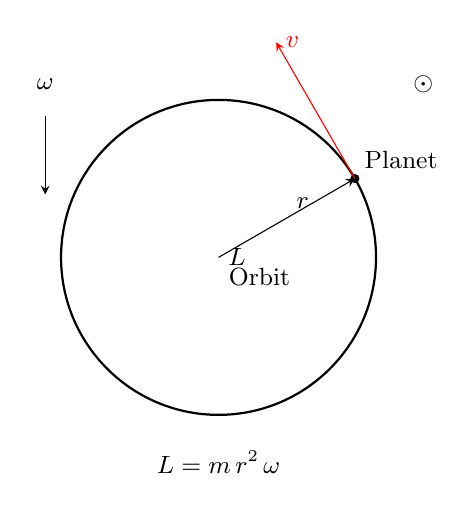
\begin{tikzpicture}[scale=2, every node/.style={font=\small}, >=stealth]
      % Center and orbit
      \coordinate (O) at (0,0);
      \draw[thick] (O) circle (1cm) node[below right] {Orbit};
  
      % Planet position
      \coordinate (P) at (0.866,0.5);
      \filldraw (P) circle (0.025cm) node[above right] {Planet};
  
      % Radius vector
      \draw[->] (O) -- (P) node[midway, above right] {$r$};
  
      % Tangential velocity vector
      \draw[->, red] (P) -- ++(-0.5,0.866) node[right] {$v$};
  
      % Angular velocity symbol (out of page)
      \node at (-1.1,1.1) {$\displaystyle \omega$};
      \draw[->] (-1.1,0.9) -- ++(0,-0.5);
  
      % Angular momentum symbol (out of page, dot in circle)
      \node at (1.3,1.1) {$\odot$} node[right] {$L$};
  
      % Formula annotation
      \node at (0,-1.3) {\(\displaystyle L = m\,r^2\,\omega\)};
    \end{tikzpicture}
    \caption{A planet of mass \(m\) at radius \(r\) with angular velocity \(\omega\) has angular momentum \(L = m r^2 \omega\), which remains constant (\(\tfrac{dL}{dt}=0\)) in the absence of external torque.}
    \label{fig:kepler-angular-momentum}
\end{figure}





But observe:

\[
L = m r^2 \omega
\]
\[
\omega = \frac{d\theta}{dt}
\]

So:

\[
L = m r^2 \frac{d\theta}{dt}
\]

Dividing both sides by 2:

\[
\frac{L}{2} = \frac{1}{2} m r^2 \frac{d\theta}{dt}
\]

But the expression on the right is none other than:

\[
\frac{dA}{dt}
\]

—the rate at which area is swept out (since \( dA = \frac{1}{2} r^2 d\theta \)).

Thus:

\[
\frac{dA}{dt} = \frac{L}{2m}
\]

Kepler’s Second Law isn’t just a geometric rule—it’s the projection of angular momentum conservation 
onto the orbital plane.




\begin{figure}[H]
    \centering
    \begin{tikzpicture}[scale=1.5, every node/.style={font=\small}, >=stealth]
      % Parameters
      \def\r{2}        % radius
      \def\dtheta{30}  % small angle in degrees
  
      % Draw and shade the infinitesimal sector
      \filldraw[fill=blue!20, draw=blue] 
        (0,0) -- (\dtheta:\r) arc (\dtheta:0:\r) -- cycle;
  
      % Radii
      \draw[thick] (0,0) -- (\dtheta:\r) node[pos=0.6, above right] {$r$};
      \draw[thick] (0,0) -- (0:\r);
  
      % Arc marking the angle dθ
      \draw[->] (1,0) arc (0:\dtheta:1) node[midway, right] {$d\theta$};
  
      % Annotation with formulas
      \node at (0,-1)   {\(\displaystyle dA = \tfrac12\,r^2\,d\theta\)};
      \node at (0,-1.5) {\(\displaystyle \frac{dA}{dt} = \tfrac12\,r^2\,\frac{d\theta}{dt}
                          = \frac{L}{2m}\)};
    \end{tikzpicture}
    \caption{An infinitesimal sector of area \(dA = \tfrac12\,r^2\,d\theta\); dividing by \(dt\) shows \(\tfrac{dA}{dt} = \tfrac{L}{2m}\) via \(L = m\,r^2\frac{d\theta}{dt}\).}
    \label{fig:kepler-infinitesimal-sector}
\end{figure}








\begin{HistoricalSidebar}{From Area to Angular Momentum}

In Newton’s geometry, Kepler’s Second Law was a balance of triangles; in Euler’s mechanics, it became the balance 
of angular momentum.

\medskip

Where Newton proved that equal areas implied a central force, Euler’s framework showed that this geometric 
constancy reflected a deeper dynamical invariant: the planet resists changes to its spin around the Sun.

\medskip

In other words: Kepler’s area law and Euler’s moment of inertia are two sides of the same coin. One speaks in 
triangles; the other speaks in torque.

\end{HistoricalSidebar}



\subsubsection{A Modern Translation}

In modern physics, we state this principle succinctly:

\[
\text{No external torque} \quad \Rightarrow \quad L = \text{constant}
\]

\[
L = m r^2 \frac{d\theta}{dt}
\quad \Rightarrow \quad
\frac{dA}{dt} = \frac{L}{2m}
\]

Kepler saw the planets sweeping equal areas; Newton showed this implied a centripetal force; Euler showed that 
this was the rotational analog of inertia.

\textbf{Equal areas in equal times is angular momentum in disguise.}

It’s a reminder that what begins as geometry can, over centuries, reveal itself as dynamics.



\begin{figure}[H]
    \centering
    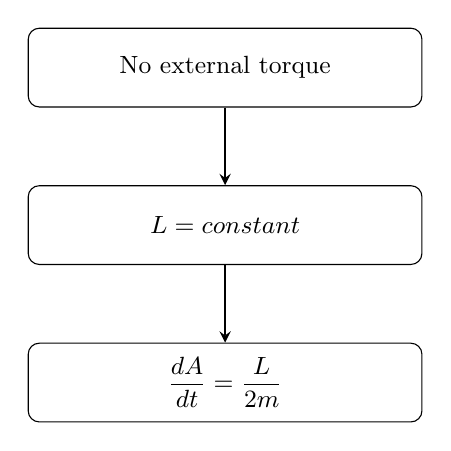
\begin{tikzpicture}[
        node distance=2cm,
        box/.style={
          draw, rectangle, rounded corners,
          align=center, font=\small,
          minimum width=5cm, minimum height=1cm
        },
        >=stealth
      ]
      % Nodes
      \node[box] (torque) {No external torque};
      \node[box] (Lconst) [below of=torque] {$L = \text{constant}$};
      \node[box] (area)   [below of=Lconst] {$\displaystyle \frac{dA}{dt} = \frac{L}{2m}$};
  
      % Arrows
      \draw[->, thick] (torque) -- (Lconst);
      \draw[->, thick] (Lconst) -- (area);
    \end{tikzpicture}
    \caption{Modern translation of Kepler’s Second Law: no torque implies constant angular momentum, which in turn yields a constant area‐sweep rate.}
    \label{fig:modern-translation-kepler}
\end{figure}
